
%!TEX program = xelatex

% Name           : demo.tex
% Author         : Moritz Flöter
% Version        : 1.0
% Created on     : 17.04.2016
% Last Edited on : 03.04.2017
% Copyright      : Copyright (c) 2016-2017 by Moritz Flöter.
% Based on       : HSRM-Theme from Benjamin Weiss
% License        : This file may be distributed and/or modified under the
%                  GNU Public License.
% Description    : HSRM beamer theme demonstration. Also includes a short 
%                  Tutorial regarding the beamer class.

%--------------------------------------------------------------------------
% aspectratio -> 4:3 -> 43, 16:9 -> 169, 16:10 -> 1610 etc.
%--------------------------------------------------------------------------
\documentclass[compress, aspectratio=43, noserifmath]{beamer}
%--------------------------------------------------------------------------
% Common packages
%--------------------------------------------------------------------------
\usepackage[german]{babel}
\usepackage{minted}
\usepackage{graphicx}
\usepackage{multicol}
\usepackage{listingsutf8}
% Erweiterte Tabellenfunktionen
\usepackage{tabularx,ragged2e}
\usepackage{booktabs}
% Listingserweiterung
\usepackage{listings}
\lstset{ %
language=[LaTeX]TeX,
basicstyle=\normalsize\ttfamily,
keywordstyle=,
numbers=left,
numberstyle=\tiny\ttfamily,
stepnumber=1,
showspaces=false,
showstringspaces=false,
showtabs=false,
breaklines=true,
frame=tb,
framerule=0.5pt,
tabsize=4,
framexleftmargin=0.5em,
framexrightmargin=0.5em,
xleftmargin=0.5em,
xrightmargin=0.5em
}

%--------------------------------------------------------------------------
% Load theme
%--------------------------------------------------------------------------
\usetheme{freshroboto}


% must be loaded after theme
\usepackage{tikz}
\usetikzlibrary{mindmap,backgrounds}

%--------------------------------------------------------------------------
% General presentation settings
%--------------------------------------------------------------------------
\title{Prototypical Realization and Validation of an Incremental Software Product Line Analysis Approach}
\subtitle{Pr\"asentation zur Masterarbeit}
\date{Letztes Update: \today}
\author{Moritz Fl\"oter}
\institute{\textbf{Universit\"at Hildesheim}}

%--------------------------------------------------------------------------
% Notes settings
%--------------------------------------------------------------------------
\setbeameroption{show notes}

\begin{document}
%--------------------------------------------------------------------------
% Titlepage
%--------------------------------------------------------------------------

\maketitle

%\begin{frame}[plain]
%	\titlepage
%\end{frame}

%--------------------------------------------------------------------------
% Table of contents
%--------------------------------------------------------------------------
\section*{Gliederung}
\begin{frame}{Gliederung}
	% hideallsubsections ist empfehlenswert für längere Präsentationen
	\tableofcontents[hideallsubsections]

\end{frame}


\section{Idee \& Motivation}
\subsection{Idee \& Motivation}

\begin{frame}{Ausgangssituation}
\begin{itemize}
        \item[\textbullet] Analysen unterst\"utzen Softwareentwicklung
        \item[\textbullet] Analysen f\"ur Software Produktlinien (SPL) sind rechenintensiv
        \item[\textbullet] Relativ sp\"ate Verf\"ugbarkeit von Ergebnissen
        \item[\textbullet] Entwickler macht mittlerweile was anderes
\end{itemize}
\end{frame}


\begin{frame}{Idee}
Inkrementelle Analysen
\begin{itemize}
    \item[\textbullet] Nicht jedes mal alles neu analysieren
    \item[\textbullet] \"Uber eingef\"uhrte Ver\"anderungen bestimmen, welcher Teil analysiert werden muss 
\end{itemize}

Umsetzung auf Basis von KernelHaven

\end{frame}



\section{Grundlagen}
\subsection{Grundlagen}

\begin{frame}{Linux Build System}
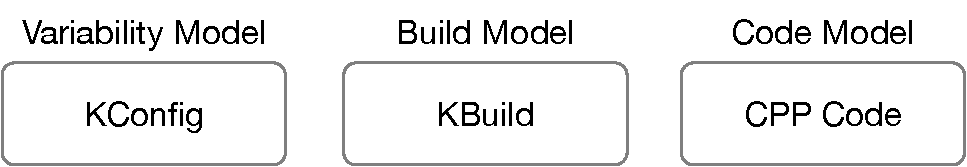
\includegraphics[width=1\textwidth]{image/linux-build-system.pdf}
\end{frame}


\begin{frame}[containsverbatim]{Variabilit\"at - Variability Model}

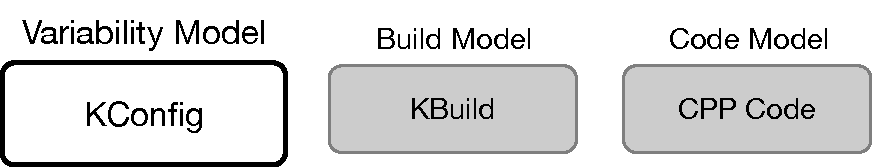
\includegraphics[width=0.8\textwidth]{image/linux-build-system-1.pdf}
\begin{minted}{kconfig}
config NETWORK_AUTHENTICATION
    bool "Network Authentication"
    depends on USER_AUTHENTICATION
    select NETWORK_SUPPORT
    default y
    help
      Network authentication support ...

\end{minted}
\end{frame}


\begin{frame}[containsverbatim]{Variabilit\"at - Build Model}
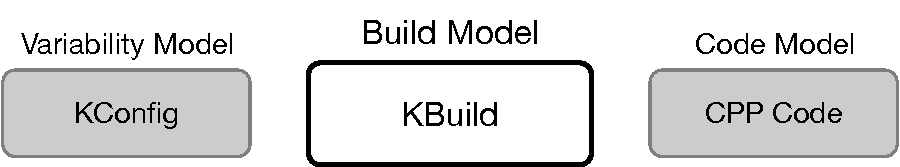
\includegraphics[width=0.8\textwidth]{image/linux-build-system-2.pdf}
\begin{minted}{make}
# Makefile for network device drivers.
obj-$(CONFIG_NETWORK_SUPPORT) += generic-driver.o
obj-$(CONFIG_NETWORK_SUPPORT) += other-drivers/
\end{minted}

\begin{minted}{make}
# Beispiel: NETWORK_SUPPORT wurde ausgewaehlt
obj-y += generic-driver.o
obj-y += other-drivers/
\end{minted}
\end{frame}



\begin{frame}[containsverbatim]{Variabilit\"at - Code Model}
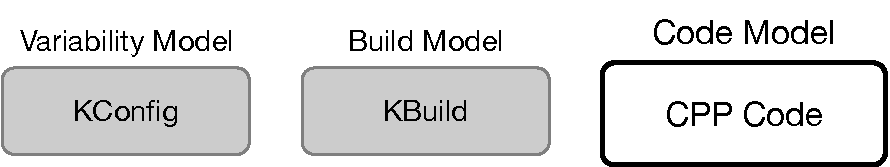
\includegraphics[width=0.8\textwidth]{image/linux-build-system-3.pdf}
\begin{minted}{cpp}
 #ifdef CONFIG_NETWORK_SUPPORT
   return 0;
 #else 
   return 1;
 #endif
\end{minted}
\end{frame}





\begin{frame}{KernelHaven}
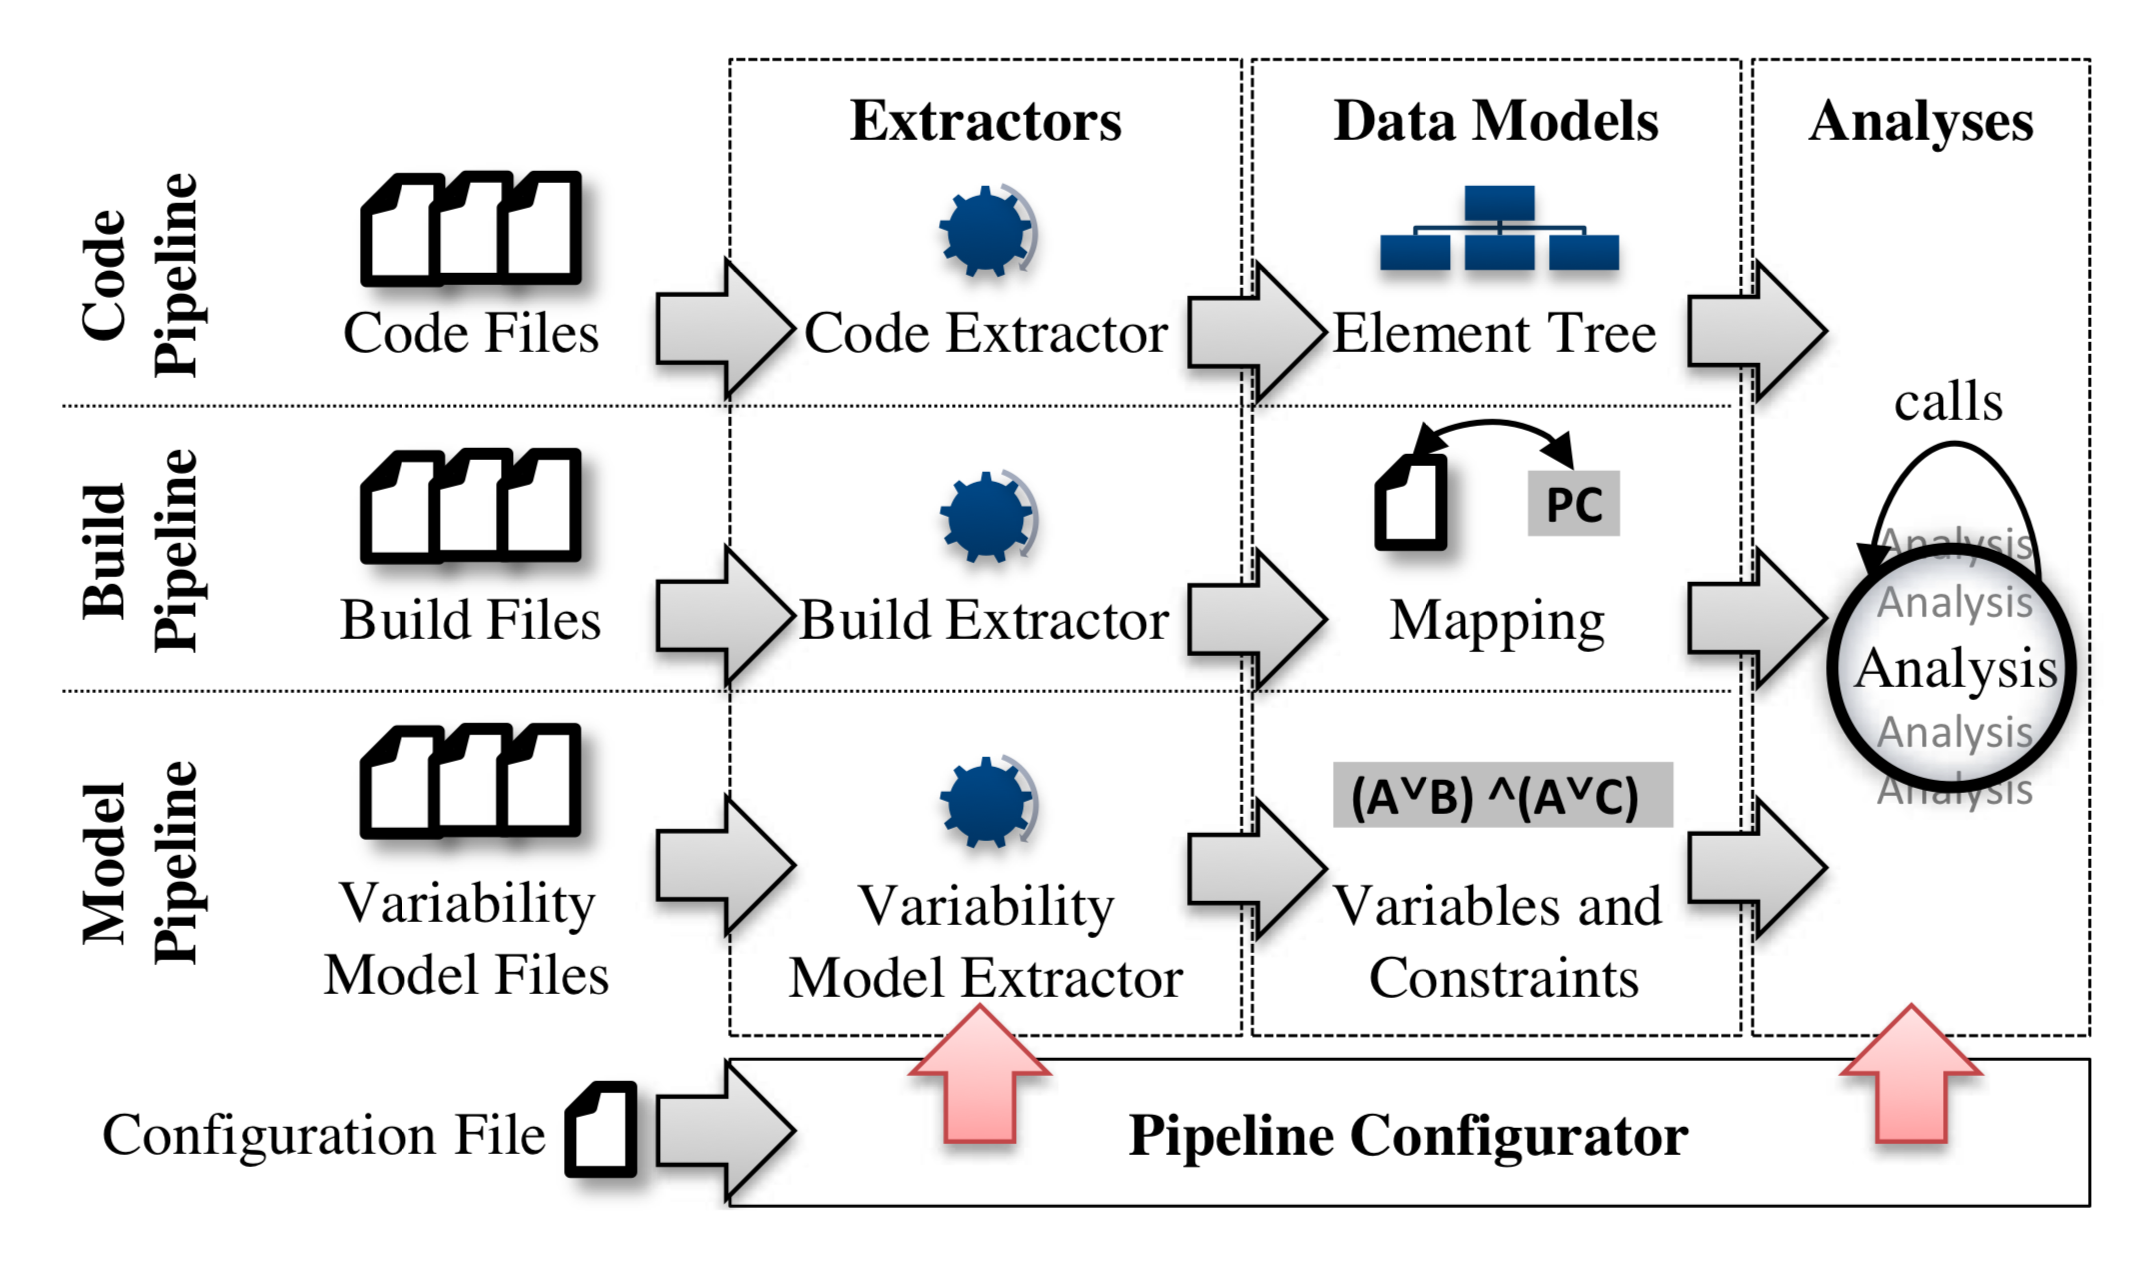
\includegraphics[width=1\textwidth]{image/KernelHaven-Pipeline}
\end{frame}

\begin{frame}[containsverbatim]{Dead Code Analyse - SPL}

\begin{minted}{python}
#ifdef CONFIG_NETWORK_AUTHENTICATION
  #ifdef !CONFIG_NETWORK_SUPPORT
    printf("You can not sign in");
  #endif
#endif
\end{minted}
\begin{minted}{kconfig}
config NETWORK_AUTHENTICATION
	bool "Network Authentication"
	...
	select NETWORK_SUPPORT
	...
\end{minted}
\end{frame}

\section{Konzept \& Implementierung}
\subsection{Konzept \& Implementierung}

\begin{frame}{Reduzierung des Aufwands}

Neu eingef\"uhrte Ver\"anderungen bestimmen, was erneut verarbeitet werden muss.
\begin{enumerate}
	\item Extraktion \\
	\emph{Die Extraktion der Modelle muss nicht vollst\"andig neu durchgef\"uhrt werden}
	\item Analyse \\
	\emph{Die Analyse muss nicht vollst\"andig neu durchgef\"uhrt werden}
\end{enumerate}
\end{frame}

\begin{frame}{Besondere Anforderungen}
Im Vorfeld wuden Anforderungen an die Implementierung festgelegt.
Dazu geh\"oren unter anderem:
\begin{itemize}
	\item[\textbullet] Rollback
	\item[\textbullet] Unterst\"utzung von Block-basierten Analysen
	\item[\textbullet] Konkrete Umsetzung von Dead Code Analyse
\end{itemize}
\end{frame}



\begin{frame}{Nicht inkrementelle Analysen}
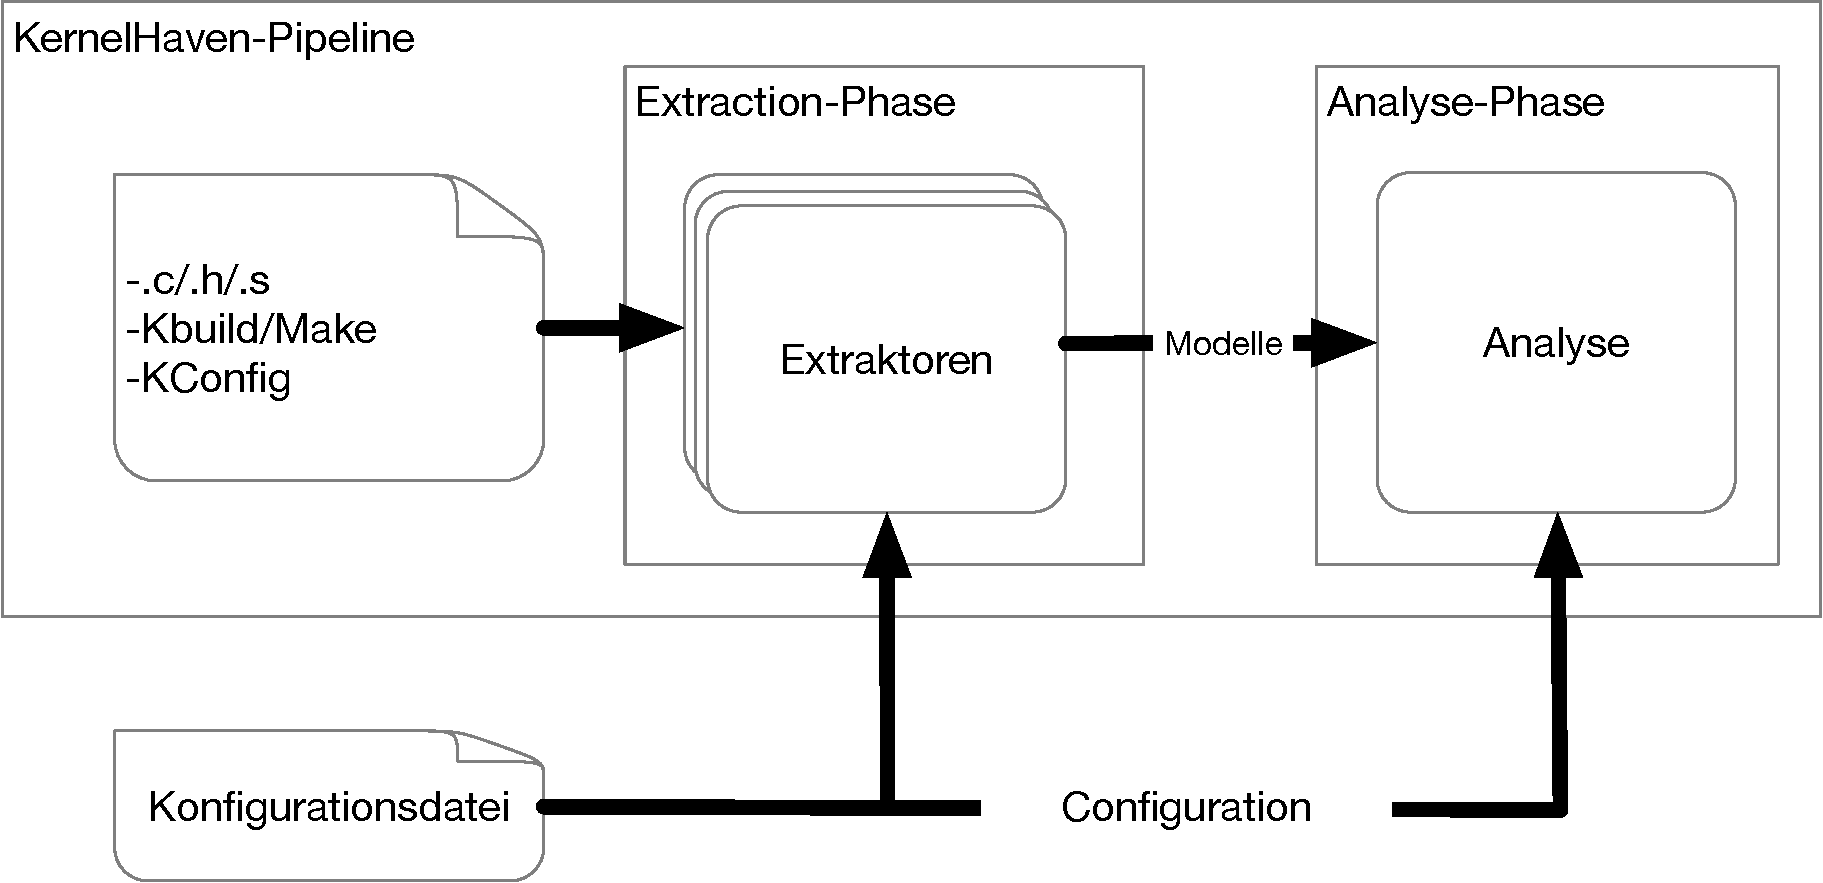
\includegraphics[width=1\textwidth]{image/KernelHaven.pdf}
\end{frame}


\begin{frame}{Inkrementelle Analysen}
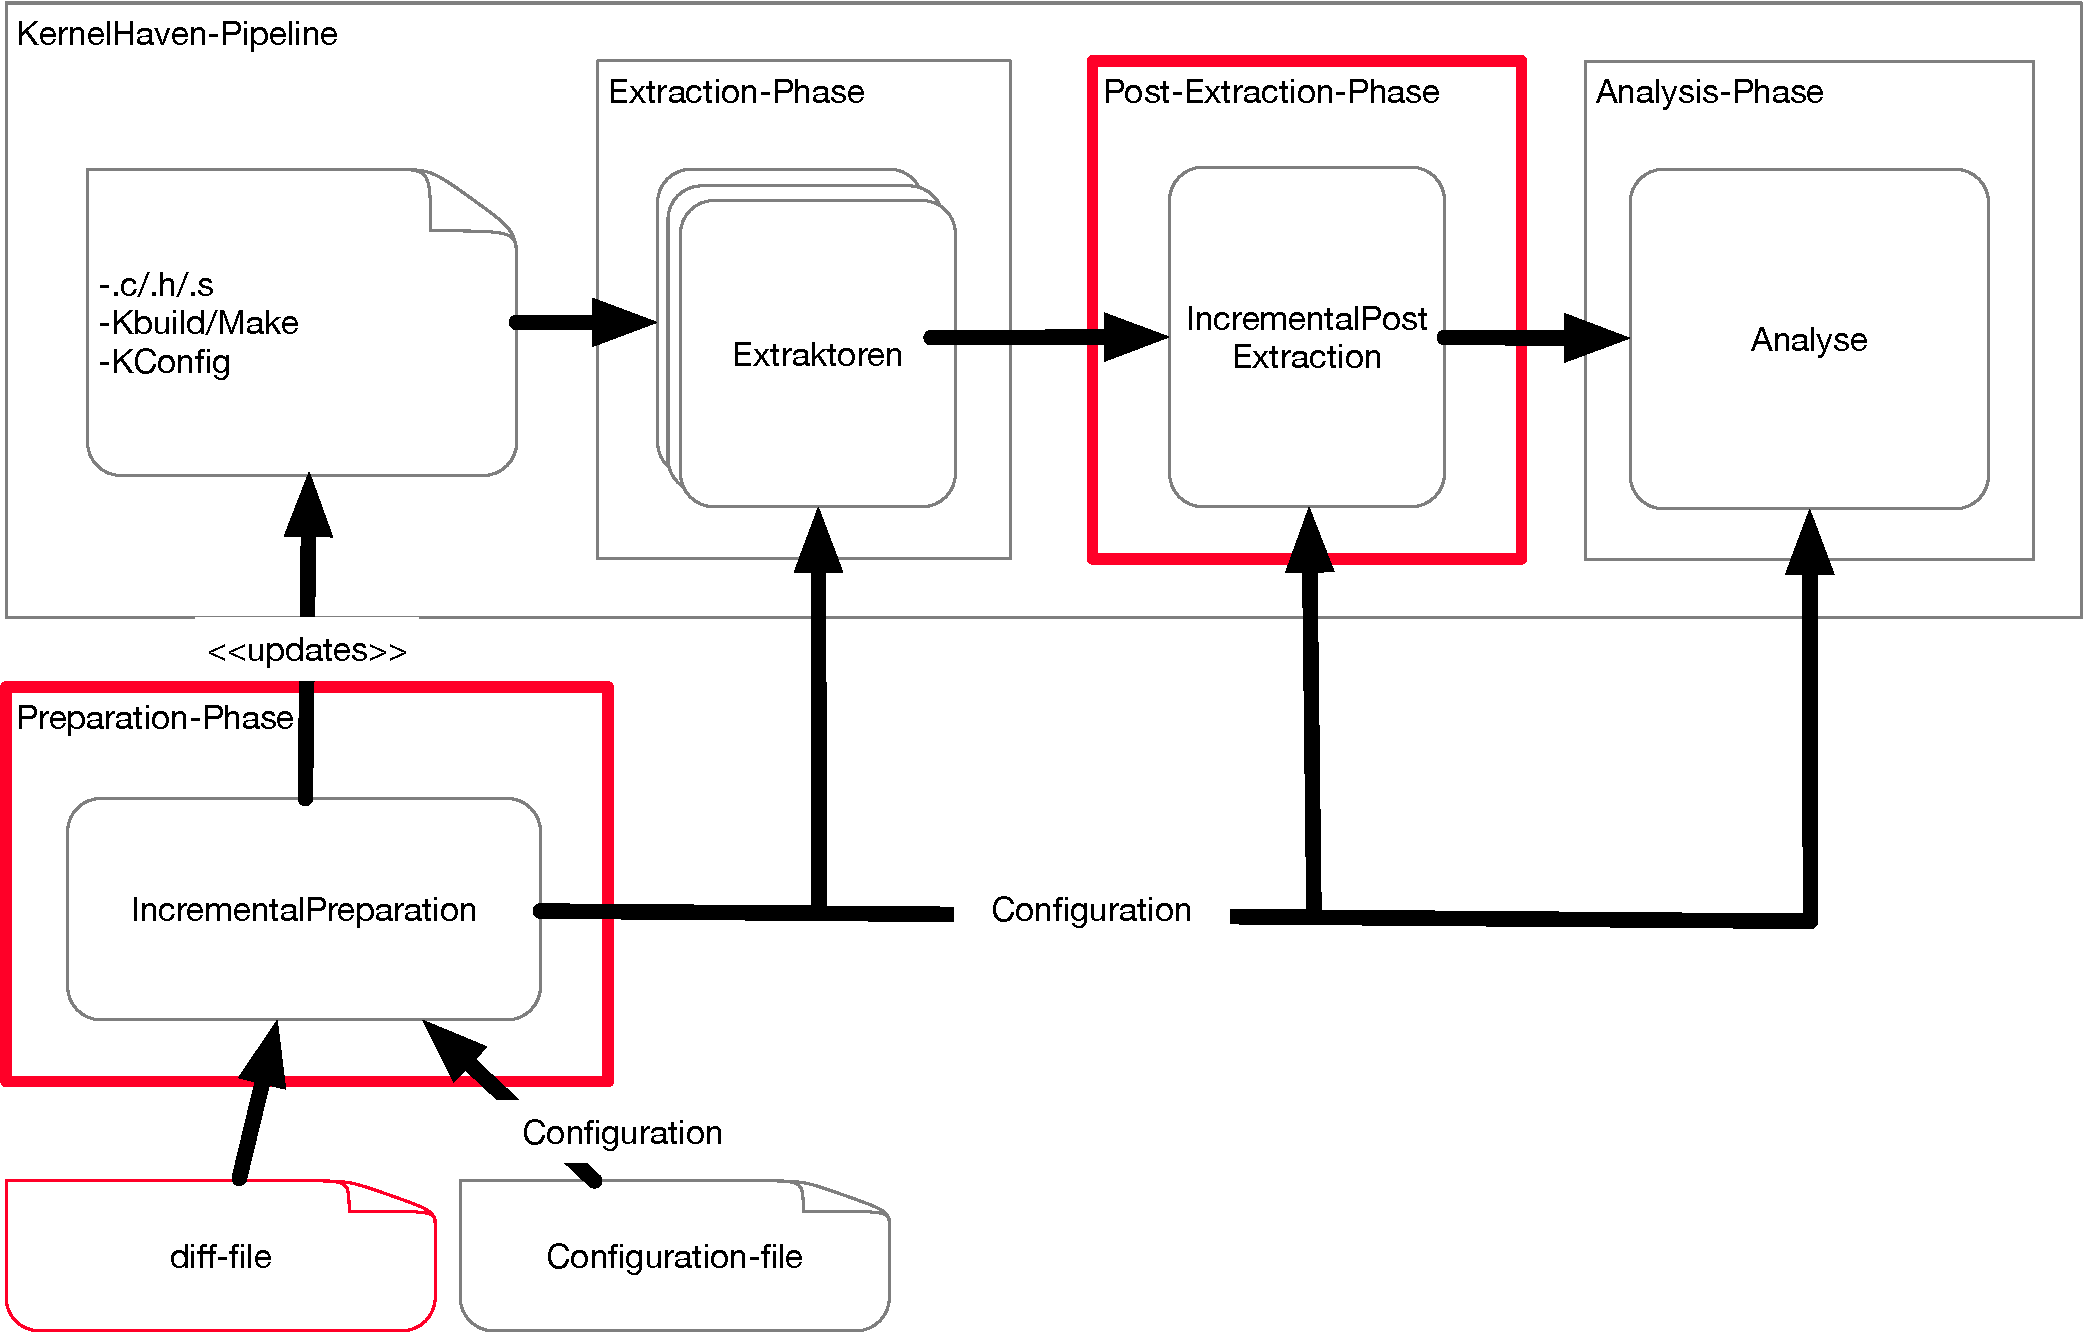
\includegraphics[width=1\textwidth]{image/KernelHavenIncremental.pdf}
\end{frame}


\begin{frame}{Preparation-Phase}
\begin{itemize}
    \item[\textbullet] Umsetzung als Preparation-Plugin
    \item[\textbullet] Aufgaben der Preparation-Phase \\
    \begin{enumerate}
       \item Anwenden der \"Anderungen auf die Codebase
       \item Filtern von Dateien f\"ur Extraktion
       \item Anpassen der Konfiguration
    \end{enumerate}
\end{itemize}
\end{frame}

\begin{frame}[containsverbatim]{Preparation-Phase}
1. Anwenden der \"Anderungen auf die Codebase

\begin{minted}{shell}
$ git apply path/to/git.diff
$ git apply --reverse path/to/git.diff
\end{minted}

\end{frame}

%TODO: �berg�nge fixen
\begin{frame}[containsverbatim]{Preparation-Phase}
2. Filtern von Dateien f\"ur Extraktion \\
Filter arbeiten auf Basis von folgenden Informationen:
\begin{itemize}
    \item[\textbullet] Dateiver\"anderung \\ \emph{Hinzuf\"ugen, Modifizieren, L\"oschen}
    \item[\textbullet] Variabilit\"ats\"anderung \\ \emph{Wurde Variabilit\"atsinformation ver\"andert?}
    \item[\textbullet] Codebase \\ \emph{Ein Filter hat Zugriff auf alle Dateien in der Codebase}
    \item[\textbullet] Regul\"arer Ausdruck \\ \emph{Welche Dateien (*.c/*.h/KConfig etc.) sollen ber\"ucksichtigt werden?}
\end{itemize}
\end{frame}

\begin{frame}[containsverbatim]{Preparation-Phase - Filtertypen}

Jeder Filter gibt eine Liste von Dateien zur\"uck, welche f\"ur die Extraktion ber\"ucksichtigt werden.

Code, Build und Variability Dateien werden separat gefiltert.

Umgesetzte Filter:

\begin{itemize}
    \item[\textbullet] \texttt{DefaultFilter} 
    \item[\textbullet] \texttt{ChangeFilter}
    \item[\textbullet] \texttt{VariabilityChangeFilter}
\end{itemize}

\end{frame}

\begin{frame}[containsverbatim]{Preparation-Phase}

3. Anpassen der Konfiguration \\

\begin{itemize}
    \item[\textbullet] Liste von Build Dateien nicht leer \\ $\rightarrow$ Build Model \alert{komplett} neu extrahieren
    \item[\textbullet] Liste von Variability Dateien nicht leer \\ $\rightarrow$ Variability Model \alert{komplett} neu extrahieren
    \item[\textbullet] Liste von Code Dateien nicht leer \\ $\rightarrow$ Code Model \alert{f\"ur diese Dateien} neu extrahieren
\end{itemize}
\end{frame}


\begin{frame}[containsverbatim]{Inkrementelle Analysen}
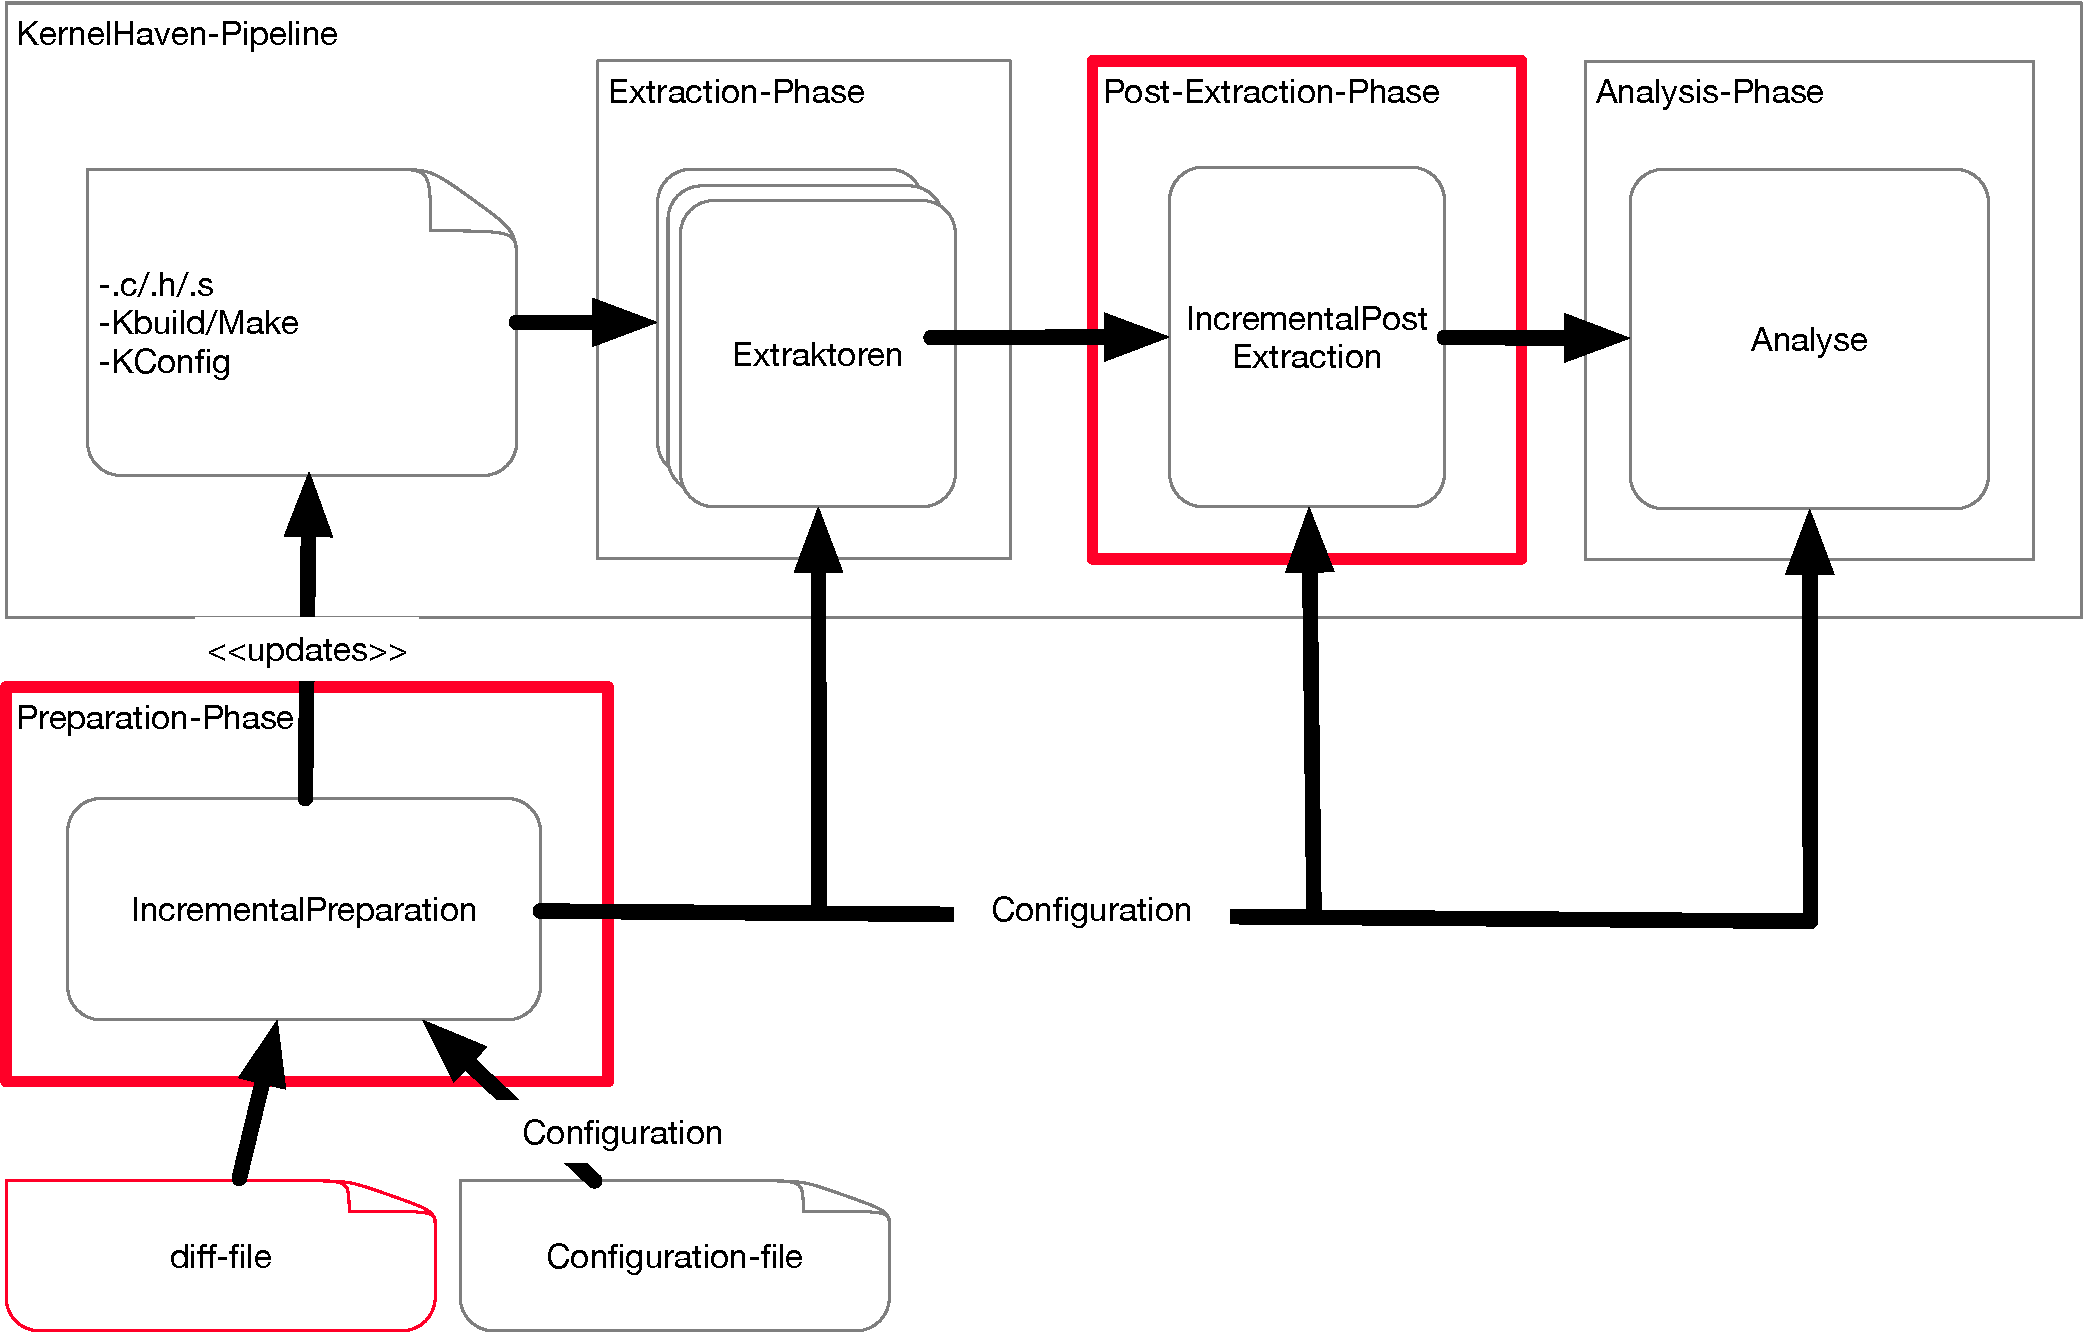
\includegraphics[width=1\textwidth]{image/KernelHavenIncremental.pdf}
\end{frame}

\begin{frame}[containsverbatim]{Post-Extraction-Phase}

\begin{itemize}
    \item[\textbullet] Umsetzung als AnalysisComponent
    \item[\textbullet] Aufgaben der PostExtraction-Phase \\
    \begin{enumerate}
       \item Einholen der Ergebnisse von Extraktoren
       \item Zusammenf\"uhren mit Ergebnissen der vorigen Extraktion
    \end{enumerate}
\end{itemize}
\end{frame}


\begin{frame}[containsverbatim]{Post-Extraction-Phase}

1. Einholen der Ergebnisse von Extraktoren

\texttt{extractor.getNextResult();}

\end{frame}

\begin{frame}[containsverbatim]{Post-Extraction-Phase}

2. Zusammenf\"uhren mit Ergebnissen der vorigen Extraktion

Konzept des HybridCache:
\begin{itemize}
    \item Ausgangssituation: \\ 
    \begin{itemize}
        \item[\textbullet]  Ordner 'current' enth\"alt Modelle zum vorigen Stand der Codebase
    \end{itemize}
    \item Verarbeitung der neuen Ergebnisse: \\
    \begin{itemize}
        \item[\textbullet] neu extrahierte Modelle ersetzen bisherige Modelle 
        \item[\textbullet] ersetzte Modelle werden in 'history'-Ordner verschoben
    \end{itemize}
\end{itemize}


\end{frame}


\begin{frame}[containsverbatim]{Post-Extraction-Phase}

Was leistet der HybridCache?
\begin{itemize}
    \item[\textbullet] Verwaltung von (bis zu) zwei Versionen der Modelle
    \item[\textbullet] Information \"uber neu extrahierte Modelle
    \item[\textbullet] Identifizierung von ver\"anderten Teilen innerhalb der Modelle
\end{itemize}
\end{frame}

\section{Dead Code Analyse}
\subsection{Dead Code Analyse}

\begin{frame}{Dead Code Analyse - Ausgangssituation}

\begin{itemize}
    \item[\textbullet] nicht inkrementelle Variante existiert bereits
    \item[\textbullet] HybridCache ist bei bestehender Implementierung nicht als Input m\"oglcih
\end{itemize}
\end{frame}


\begin{frame}{Hybrid Cache Adapter}
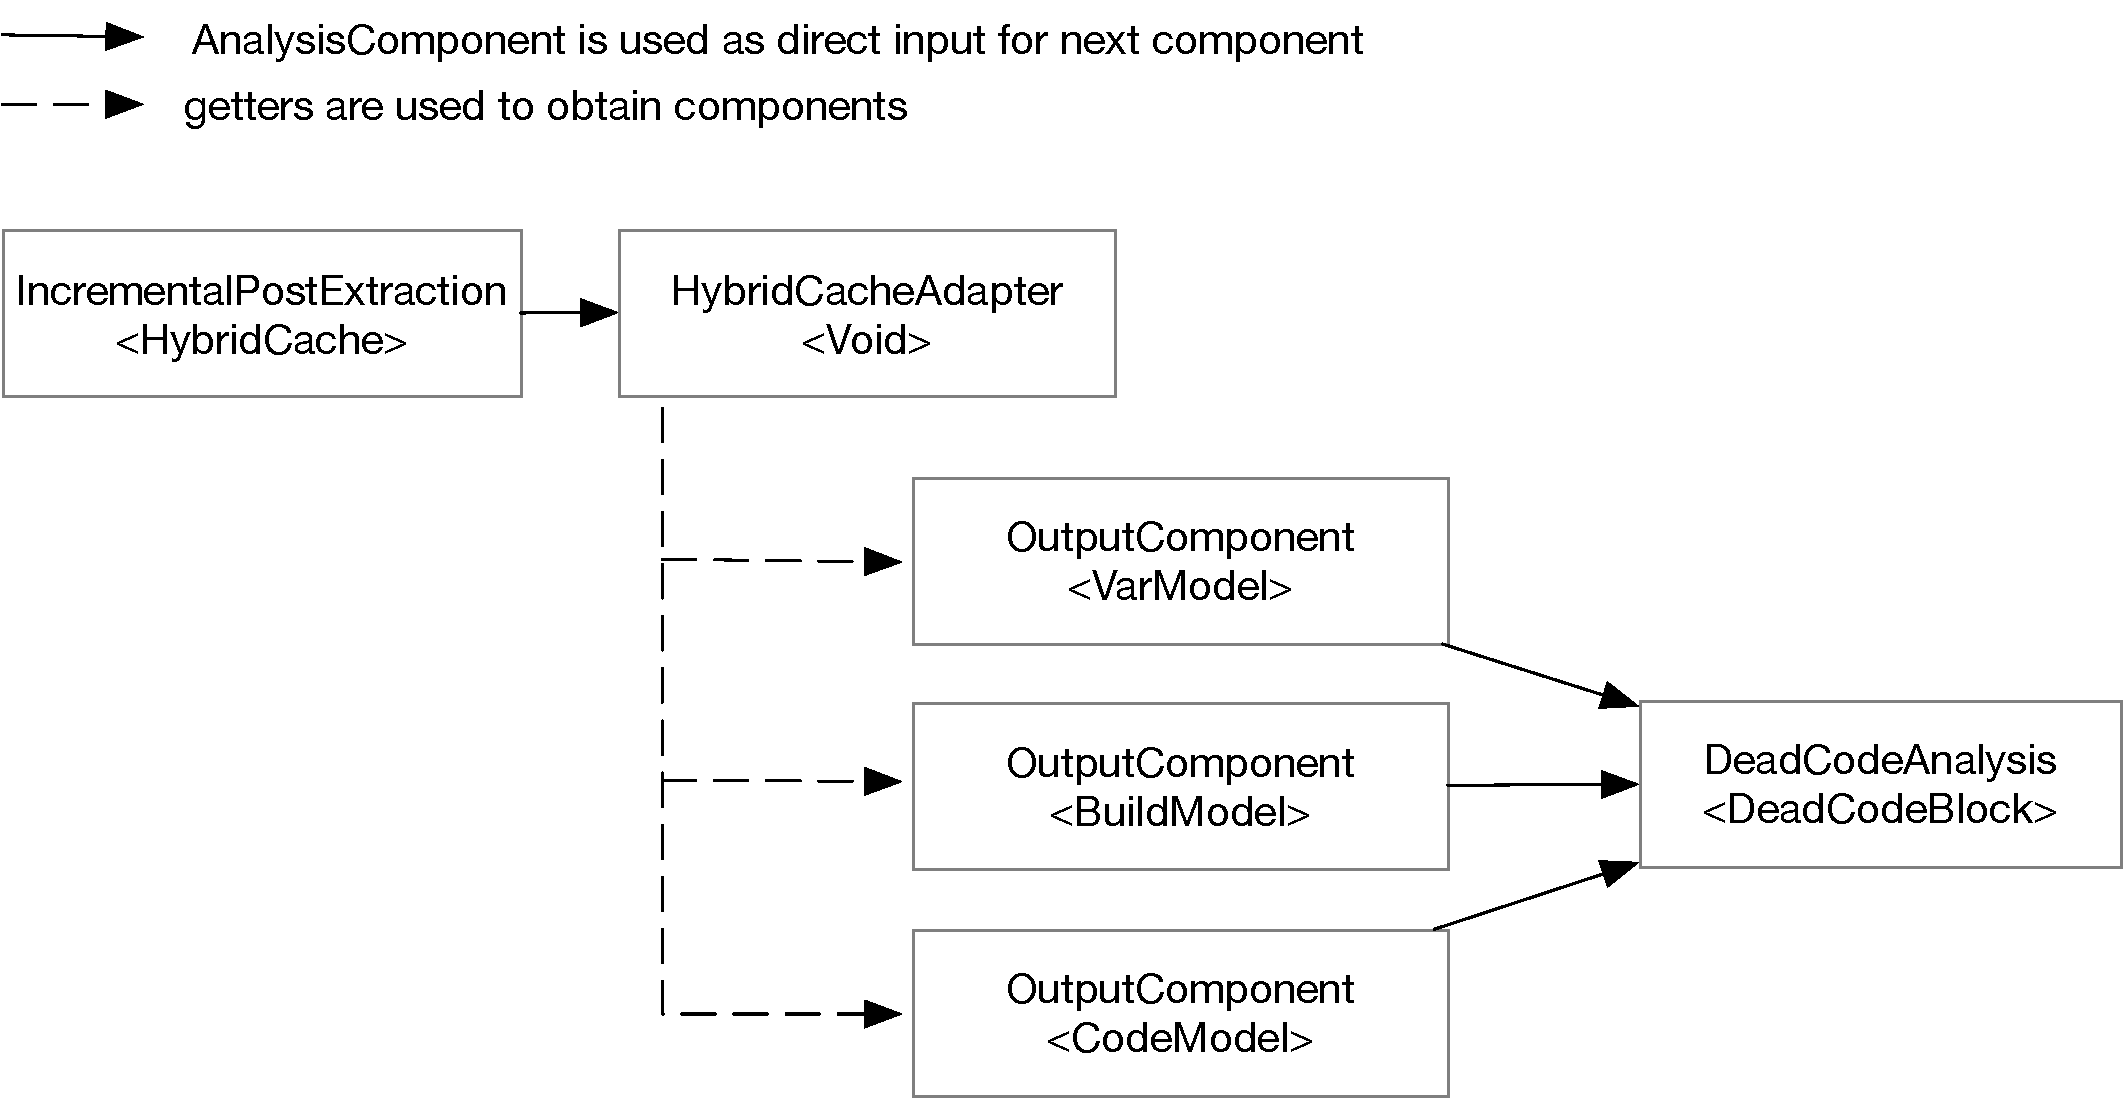
\includegraphics[width=1\textwidth]{image/HybridCacheAdapter.pdf}
\end{frame}

\begin{frame}{Hybrid Cache Adapter}
Das Code Model kann
\begin{itemize}
    \item[a)] komplett
    \item[b)] partiell (nur f\"ur neu extrahierte Dateien)
\end{itemize}
weitergegeben werden.
\end{frame}

\begin{frame}{Dead Code Analyse}
Die Dead Code Analyse verarbeitet das Code Model 
\begin{itemize}
    \item[a)] komplett \\
    \emph{wenn variability oder build model \alert{ver\"andert} wurden}
    \item[b)] partiell (nur f\"ur neu extrahierte Dateien)
    \emph{wenn variability oder build model \alert{nicht ver\"andert} wurden}
\end{itemize}
weitergegeben werden.
\end{frame}

\section{Evaluation}

\subsection{Evaluation}

\begin{frame}{Evaluation}
Vier Konfigurationen:
\begin{itemize}
    \item[\textbullet] Ref
    \item[\textbullet] Change
    \item[\textbullet] VarChange
    \item[\textbullet] FilterOff
\end{itemize}
angewendet auf 306 Commits Linux Kernels (ca. 3 Monate)
\end{frame}

\begin{frame}{Evaluation - Change}

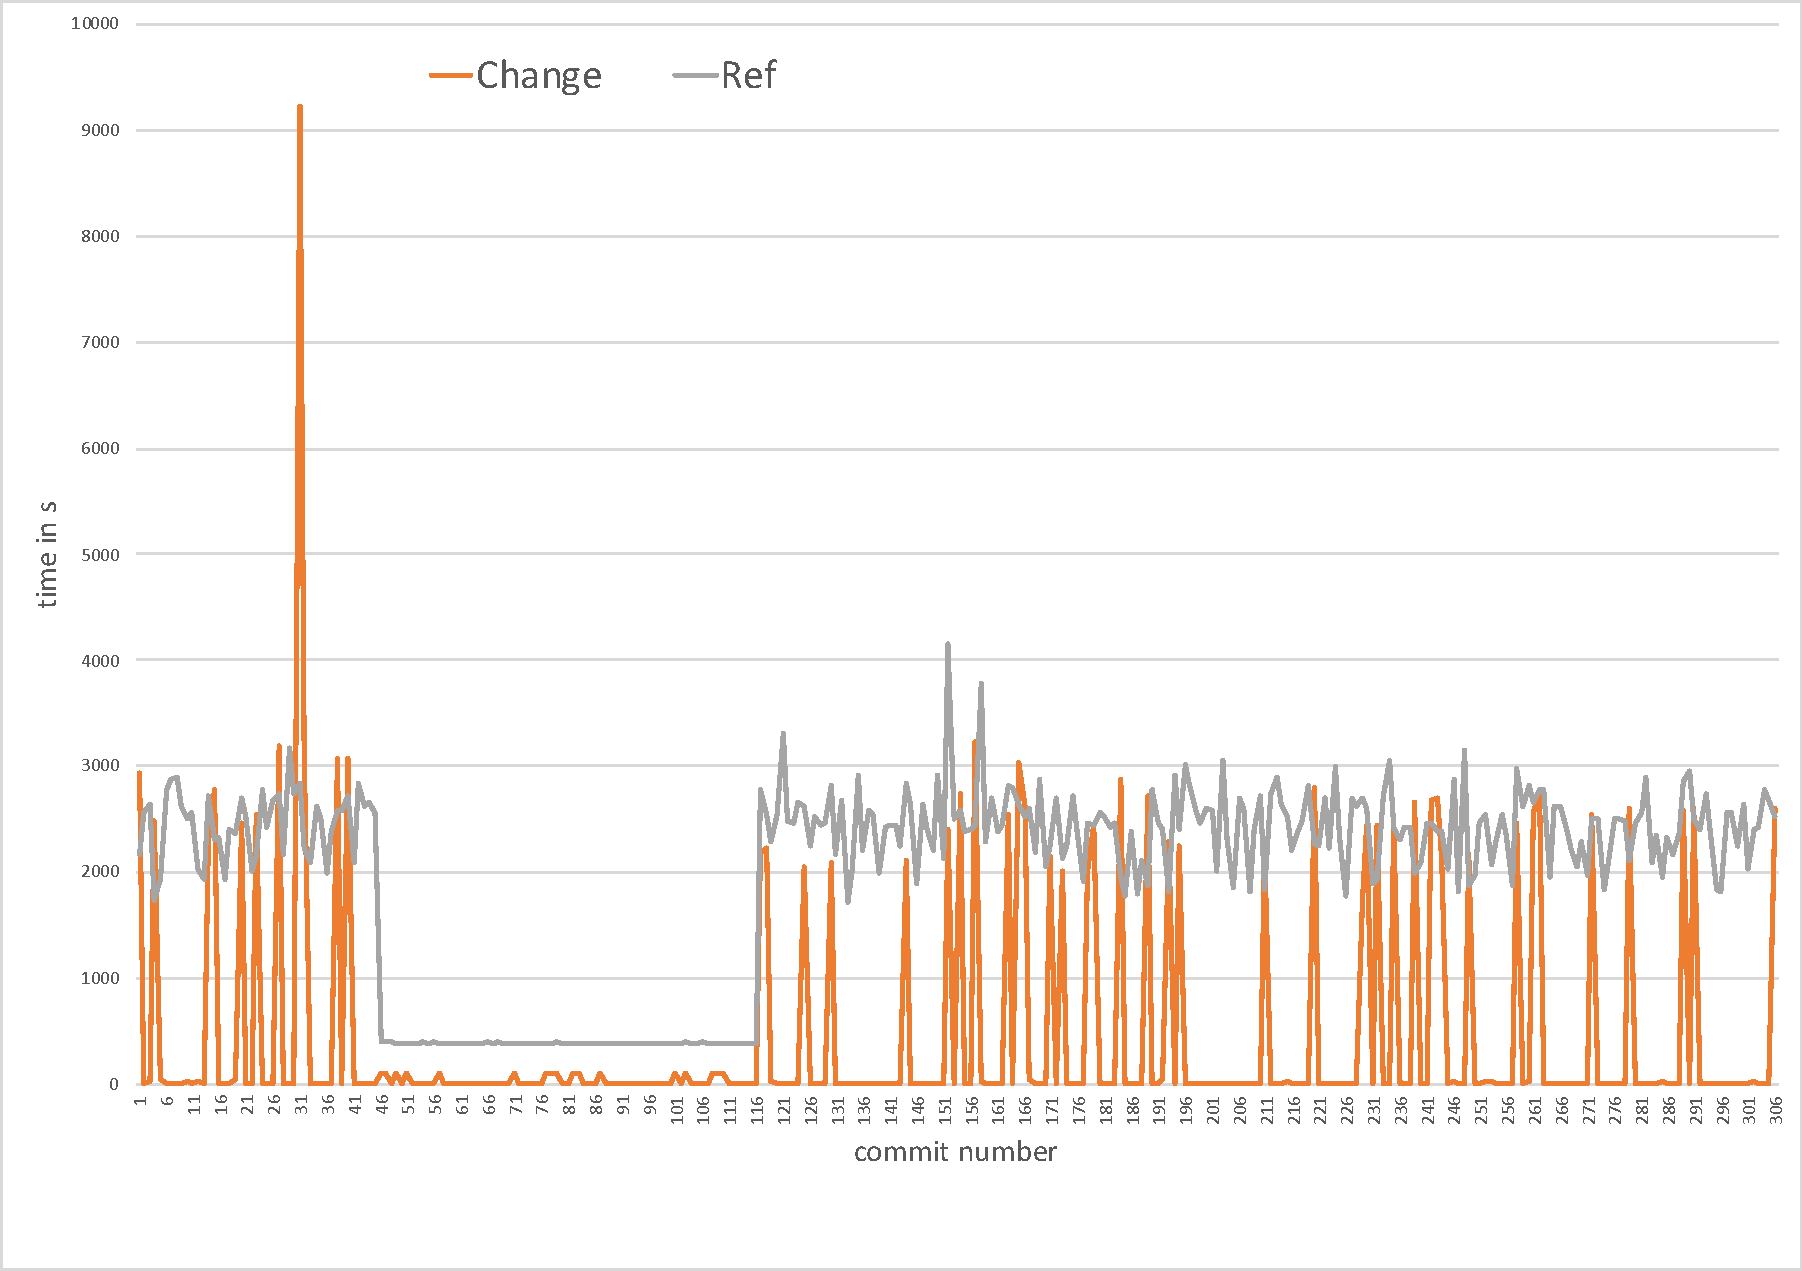
\includegraphics[width=1\textwidth]{image/change-vs-ref}

\end{frame}

\begin{frame}{Evaluation - VarChange}

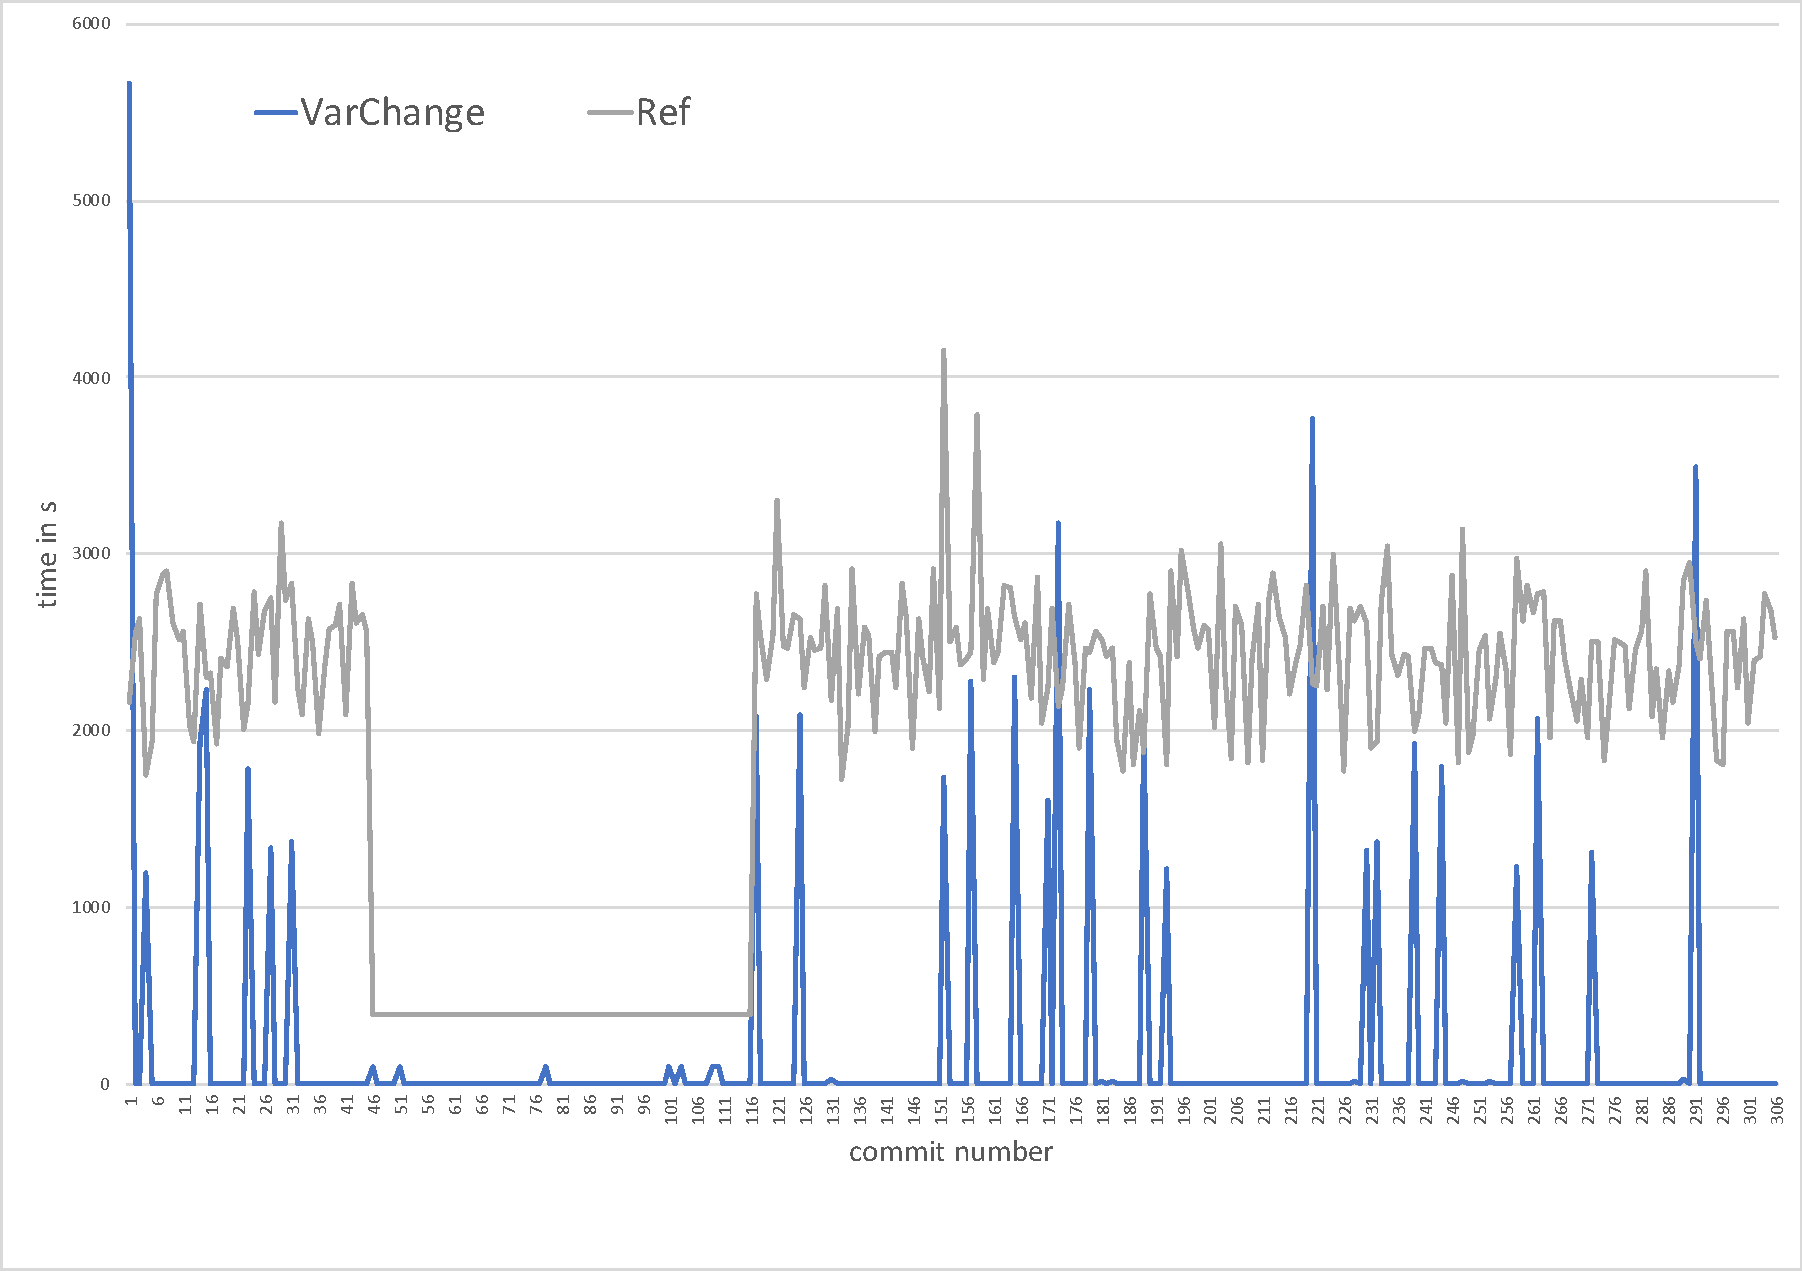
\includegraphics[width=1\textwidth]{image/var-change-vs-ref}

\end{frame}

\begin{frame}{Evaluation - Ref}

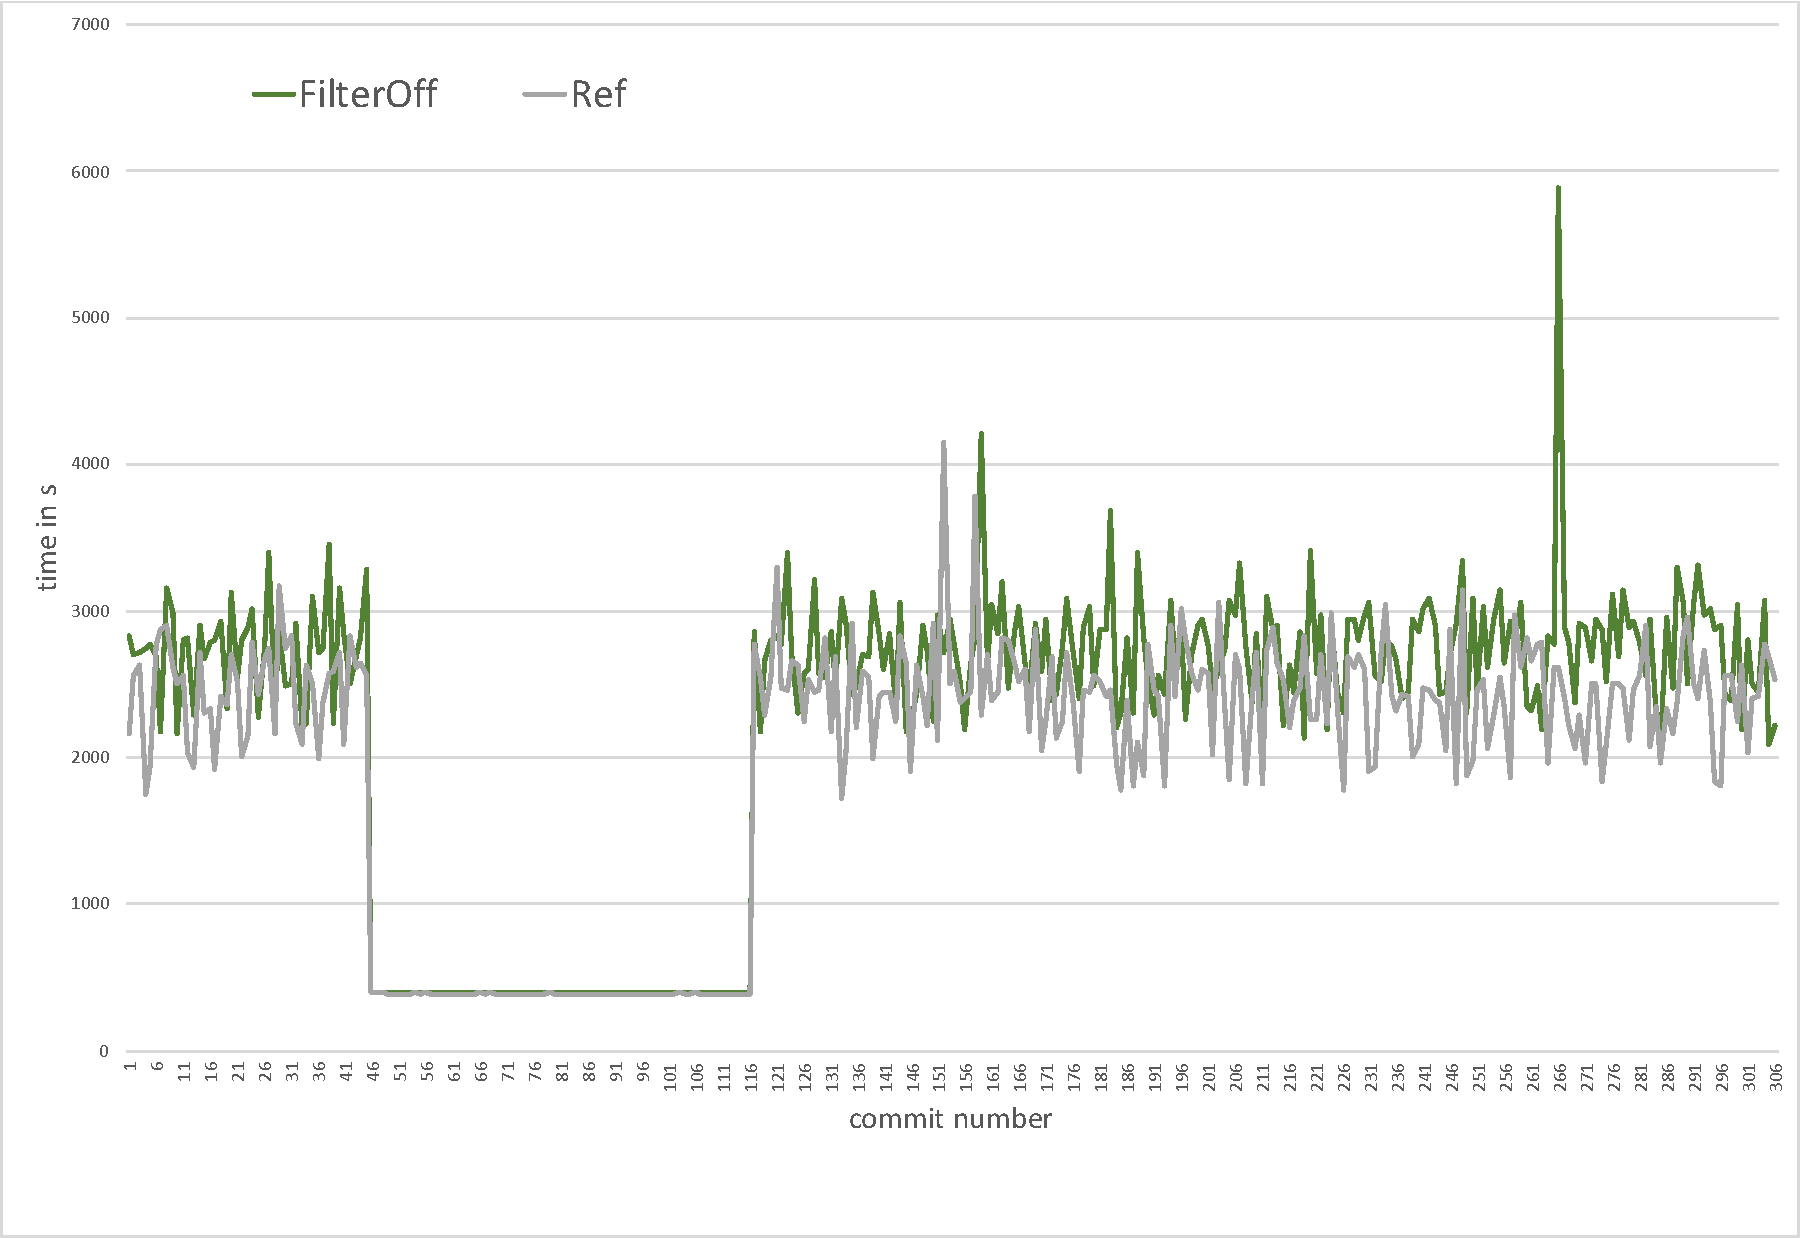
\includegraphics[width=1\textwidth]{image/filteroff-vs-ref}

\end{frame}

\begin{frame}{Evaluation - Numbers}
\begin{tabular}{|l | l | l | l|}
\hline
                               & Change                 & VarChange          & Ref  \\ \hline
	Preparation                & 0.07 s                & 11.72 s             & 0.00 s \\
	\underline{E}xtraction     & 26.22 s                & 11.70 s            & 608.80 s \\
	\underline{A}nalysis       & 407.94 s               & 157.25 s           & 1792.80 s \\
	\underline{O}verlap        & 0.00 s                 & 0.00 s             & 501.45 s \\
	E + A - O                  & 434.16 s               & 168.95 s           & 1900.15 s \\
	Post-Extraction             & 1.91 s                 & 0.50s              & 0.00 s \\ \hline
	Total                      & 7 min 16 s             & 3 min 2 s          & 32 min 47 s \\ \hline
\end{tabular}

\begin{itemize}
    \item[\textbullet] 10\% (VarChange) - 20\% (Change) brauchten l\"anger als 60 Sekunden
    \item[\textbullet] Die restlichen 80-90\% der Ausf\"uhrungen ben\"otigten im Durchschnitt 6.6s (Change) bzw. 2.3s (VarChange)
    \item[\textbullet] FilterOff war im Schnitt ca. 10\% langsamer als Ref
\end{itemize}
\end{frame}


\begin{frame}{Evaluation - Konsistenz der Ergebnisse}

\begin{itemize}
    \item Change \\
    \begin{itemize}
        \item enth\"alt alle neuen Dead Code Bl\"ocke
    \end{itemize}
    \item VarChange\\
    \begin{itemize}
        \item enth\"alt alle neuen \emph{variabilit\"atsbezogenen} Dead Code Bl\"ocke
        \item weicht teilweise in Zeilennummern der Dead Code Bl\"ocke ab
    \end{itemize}
\end{itemize}
\end{frame}

\begin{frame}{Fazit}

Inkrementelle Analysen
 
\begin{itemize}
    \item[\textbullet] 5-10fache Performanz
    \item[\textbullet]  konsistente Ergebnisse
\end{itemize}
Future Work
\begin{itemize}
    \item[\textbullet]  partielle Extraktion von Build, Variability Model
    \item[\textbullet]  Anwendung des Konzeptes auf andere Analysen
\end{itemize}
\end{frame}



\end{document}
